\begin{frame}[allowframebreaks]
    \frametitle{Pustaka 2: Tambahan}
    \justifying

    Block Radar dan Kamera:\\
    Blok radar dan kamera adalah ResNet-50 yang dimodifikasi. Blok ini memiliki dua blok konvolusi, yakni blok \textit{R-Stem} dan \textit{R-Block1}. \textit{R-Stem} adalah modul stem asli ResNet-50 untuk memproses data masukan dari sensor. R-Block1 mirip dengan tahap pertama dari ResNet-50, tetapi hanya memiliki blok residual.

    Ukuran konvolusi SAF:\\
    SAF yang paper ini usulkan terdiri dari tiga kelompok lapisan konvolusi untuk mengekstrak matriks spatial attention. Konfigurasi dalam layer "Conv $1 \times 1$" berarti ukuran kernel $1 \times 1 \times 256 \times 1$, stride $(1, 1)$, padding $[0, 0]$. Adapun lapisan "Conv $3 \times 3$" dan "Conv $5 \times 5$" konfigurasinya masing-masing
    $$
        \{3 \times 3 \times 256 \times 1, (1, 1), [1, 1]\}
        \quad dan \quad
        \{5 \times 5 \times 256 \times 1, (1, 1), [2, 2]\}
    $$

    Block RetinaNet:\\
    loss functionnya
    \begin{equation}
        L\left(c_{i}, t_{i}\right)=1 / N_{p o s} \sum_{i} L_{c l s}\left(c_{i}, c_{i^{*}}\right)+\frac{\lambda}{N_{p a s}} \sum_{i} I_{c_{i}>0} L_{r e g}\left(t_{i}, t_{i^{*}}\right)
        \label{eq: FCOS-loss-fn}
    \end{equation}

    \begin{center}        
        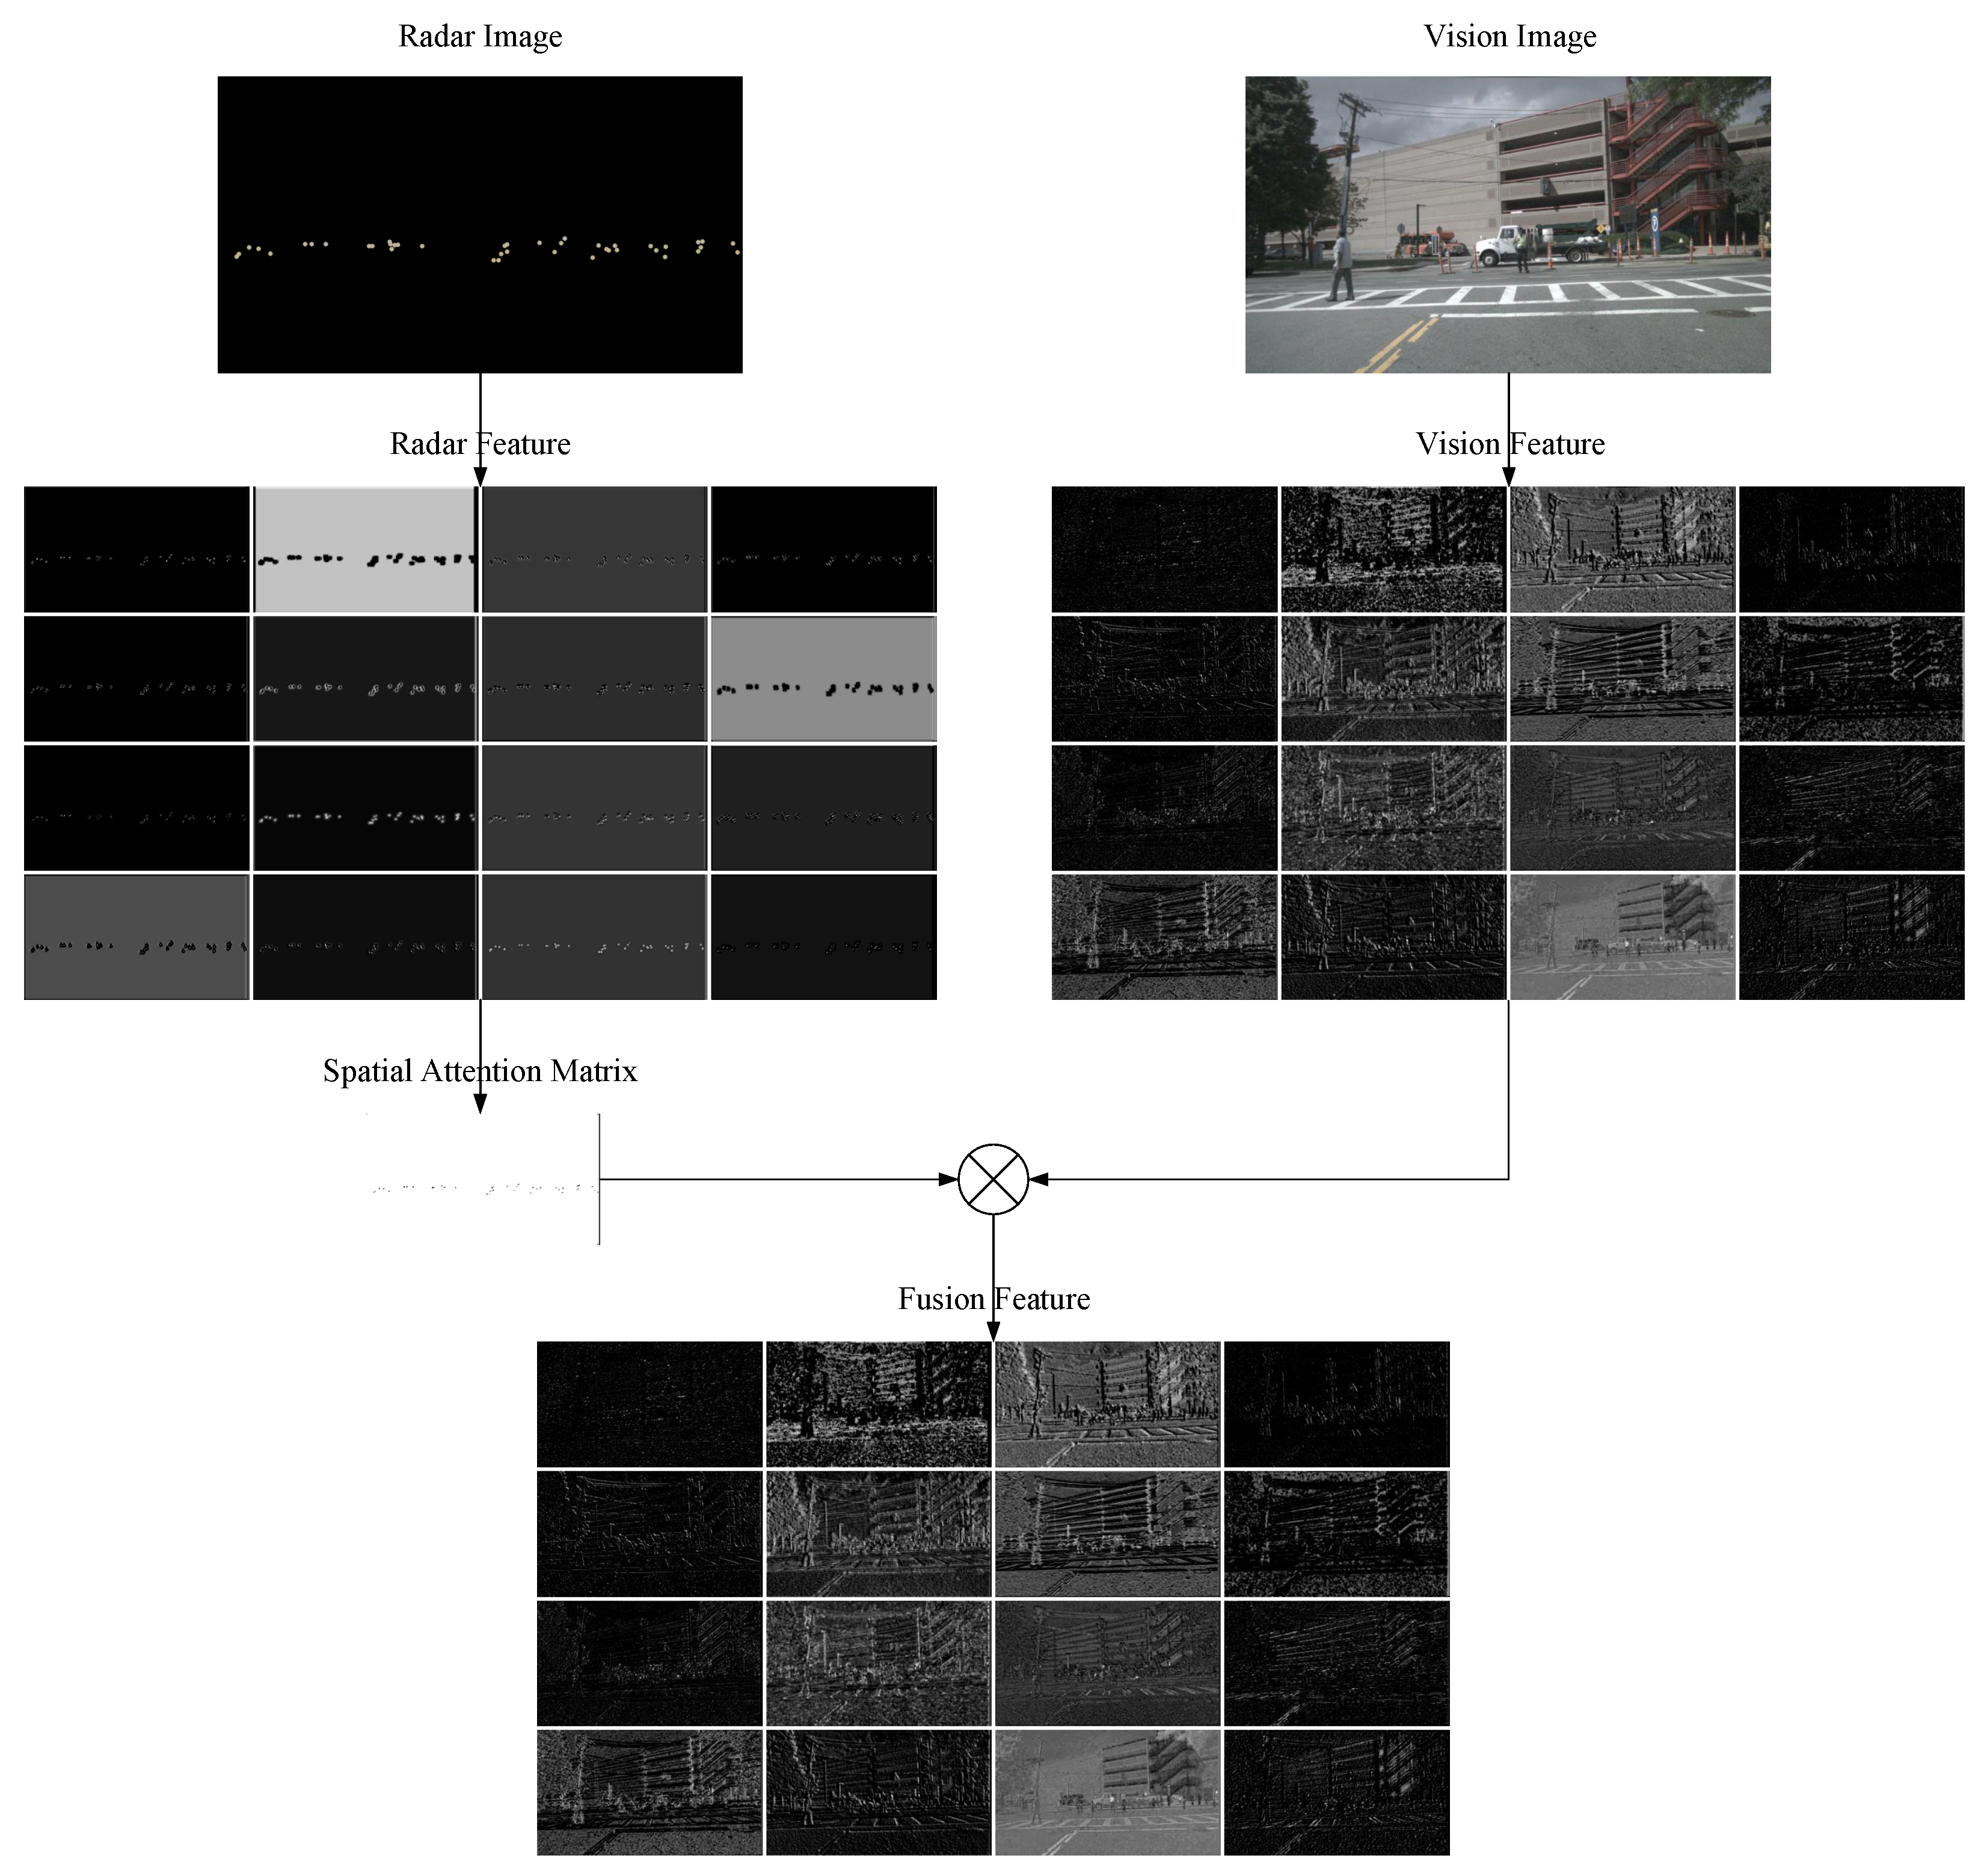
\includegraphics[width=.45\textwidth]{2-SAF-feature.png}
    \end{center}

\end{frame}